\subsection*{b. Borrar todas las órdenes de la ciudad Utah que tengan artículos de la subctegoría Tables.}
\subsubsection*{Desarrollo de operación.}
Primero, se hizo un JOIN de órdenes y productos conforme al atributo de \texttt{productid} que comparten, filtrando los productos en la subcategoría `\textit{Tables}', y se conservó solo la parte de órdenes (obteniendo un subconjunto), esto bajo el nombre de \texttt{r}.

Después, se hizo un JOIN de \texttt{r} y clientes, esto conforme al atributo de \texttt{customerid} que comparten, filtrando los clientes con vivienda en Utah, y se conservó solo la parte de órdenes (obteniendo un subconjunto), esto bajo el nombre de \texttt{s}.

Así, se tiene que \texttt{s} es la parte de \texttt{orders} con productos asociados con subcategoría `\textit{Tables}' y clientes asociados con vivienda en Utah.

Finalmente, basta con hacer la consulta con la resta de \texttt{s} a \texttt{orders} para producir la eliminación.

\addcontentsline{toc}{subsection}{b.}

Expresion:
\begin{itemize}[nosep]
\item [\ ] $r =$
    \begin{itemize}
    \item [\ ] $\pi_{orders.*}$
    \item [\ ] $($
        \begin{itemize}
            \item [\ ] $\sigma_{products.subcategory = 'Tables'}$
                \begin{itemize}
                    \item [\ ] $(orders$
                        \begin{itemize}
                            \item [\ ] $\bowtie_{orders.productid = products.productid}$
                        \end{itemize}
                    $products)$
                \end{itemize}
        \end{itemize}
    $)$
\end{itemize}
\item [\ ] $	$
$s =$
\begin{itemize}
\item [\ ] $\pi_{orders.*}$
\item [\ ] $($
    \begin{itemize}
    \item [\ ] $\sigma_{customer.state = 'Utah'}$
            \begin{itemize}
                \item [\ ] $(customer$
                    \begin{itemize}
                        \item [\ ] $\bowtie_{customer.customerid = r.customerid}$
                    \end{itemize}
                $r)$
            \end{itemize}
\end{itemize}
$)$
\end{itemize}
$	$
$orders-s$

\end{itemize}
Resultados obtenidos:
\begin{figure}[h!]
\centering
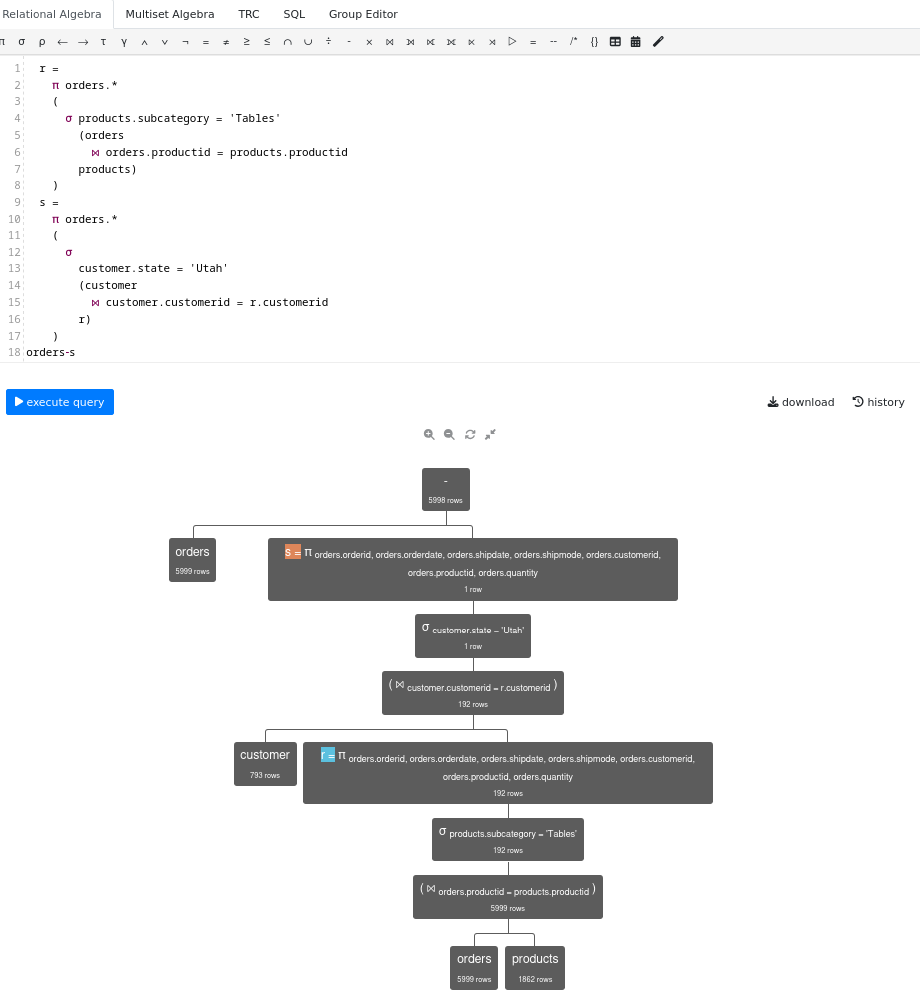
\includegraphics[width=0.8\textwidth]{imagenes/result3B1.png}
\caption{Consulta y árbol generado.}
\end{figure}

\begin{figure}[h!]
\centering
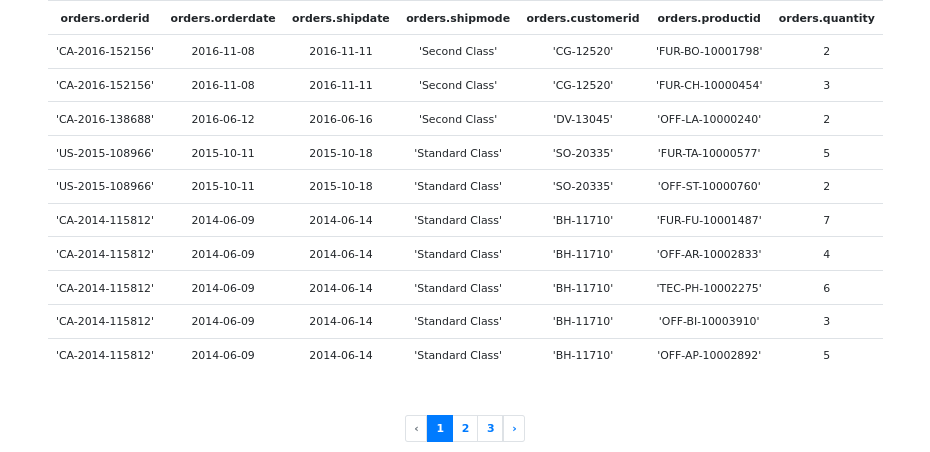
\includegraphics[width=0.8\textwidth]{imagenes/result3B2.png}
\caption{Resultado generado.}
\end{figure}
